\chapter{Testing }\label{chp4}
For the security purpose testing gives a guarantee of correctness.  It is a major chapter for assertion of the research quality. Typically our research is a part of big data and Machine learning. We used analysis and statistical testing to make sure that the results are true.

The process of extracting entities can be done in different ways. Either manually or by the use of machine learning algorithms. The manual way has many disadvantages as explained in Chapter \ref{Chapter2}.

Computer algorithms have impact for solving human problems. However we have to do a comparison for a small dataset between algorithm results and human results. The correctness of a tested dataset gives a confidence for remaining datasets.

IFRC uses the templates formats to produce their report. It is way of structuring a content of the document. The use of templates made most IFRC reports to have almost  the same size of top section. Top section contains important summary  as explained in Chapter \ref{top} .

Due to the time limitations, We tested  some  sample documents and We concluded for all top sections of the reports.
\section*{JSON file }
By taking the sample file, We extracted names of entities in JSON format. JSON stands for Java Script Object Notation. It is built based on two universal data structures such as a pair composed by a name and a value, and ordered list of values which is considered as an array, sequence, vector or list.
\begin{figure}[hbtp]
\caption{JSON File Structure}
\centering
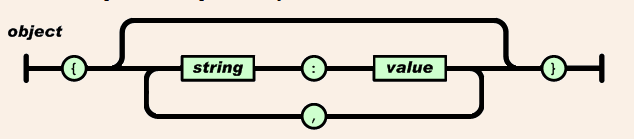
\includegraphics[scale=.7]{images/json.png}\label{json}
\end{figure}


Figure \ref{json} refers to the structure of our json file. It contains a small dictionary which has one feature of proper names. We are able to identify three people who participate in IFRC sample report.
\newpage 
\begin{figure}[hbtp]
\centering
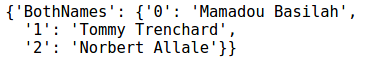
\includegraphics[scale=.7]{images/BothNames.png}
\caption{Persons Names Extracted by Hands}\label{Hand}
\end{figure}

After extracting three proper names as the Figure \ref{Hand} shows,  We are now going to do a comparison. 